Amidakuji is a custom in Japan which 
allows for a pseudo-random assignment of children to prizes~\cite{A1}. 
Usually done in Japanese schools, a teacher will draw $n$ vertical lines, 
hereby known as \emph{lines}, where $n$ is the number of students in class. 
At the bottom of each line will be a unique prize. At the top of each line will be the name of one of the students.  
The teacher will then draw 0 or more horizontal lines, hereby known as \emph{bars}, 
connecting two adjacent lines. The more bars there are the more complicated (and fun) 
the Amidakuji is. No two endpoints of two bars can be touching. Each student then traces 
their line, and whenever they encounter an end point of a bar along their line, 
they must cross the bar and continue going down the adjacent line. 
The student continues tracing down the lines and crossing bars 
until they get to the end of the ladder lottery. The prize at the bottom of the ladder lottery 
is their prize~\cite{A1}. See Figure~\ref{fig:aa} for an example of a ladder lottery.
\begin{center}
\begin{figure}[h]
	\centering
		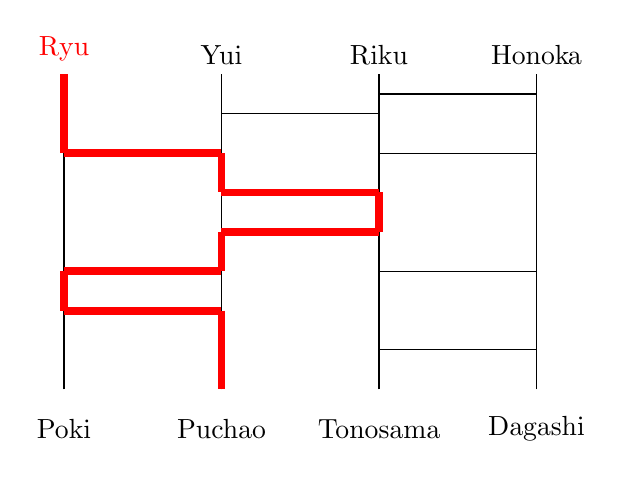
\begin{tikzpicture}
		%%Start of figure. Fig 1
			\draw(0, 0) to (0, 3); 
		
			\node at (0, -0.5){Poki};
			\draw(2, 0) to (2, 4) node[above]{Yui};
			\node at (2, -0.5){Puchao};
			\draw(4, 0) to (4, 4)node[above]{Riku};
			\node at (4, -0.5){Tonosama};
			\draw(6, 0) to (6, 4)node[above]{Honoka};
			\node at (6, -0.5){Dagashi};
			
			%bars%
		    \draw[line width=1mm, red](0, 3) to (0, 4) node[above]{Ryu};
			\draw[line width=1mm, red](0, 1) to (2, 1);
			\draw[line width=1mm, red](2, 1.5) to (2, 2);
			\draw[line width=1mm, red](0, 1)to(0, 1.5);
			\draw[line width=1mm, red](2, 1) to (2, 0);
			\draw[line width=1mm, red](0, 3) to (2, 3);
			\draw[line width=1mm, red](2, 3) to (2, 2.5);
			\draw[line width=1mm, red](4, 2) to (4, 2.5);
			\draw[line width=1mm, red](0, 1.5) to (2, 1.5);
			
			\draw[line width=1mm, red](2, 2) to (4, 2);
			\draw[line width=1mm, red](2, 2.5) to (4, 2.5);
			\draw(2, 3.5) to (4, 3.5);
			
			\draw(4, 0.5) to (6, 0.5);
			\draw(4, 3) to (6, 3);
			\draw(4, 1.5) to (6, 1.5);
			\draw(4, 3.75) to (6, 3.75);
		\end{tikzpicture}
\caption{\tiny{A ladder lottery where Ryu gets Puchao, Yui gets Dagashi, Riku gets Tonosama and Honoka gets Poki}}
\label{fig:aa}
\end{figure}
\end{center}
The game of Amidakuji has an interesting history. Amida is the Japanese name 
for Amithaba, the supreme Buddha of the Western Paradise. Amithaba
was a Buddha from India and there was a cult based around him. The cult 
of Amida, otherwise known as Amidism, believed that by worshiping Amithaba, they would 
enter into his Western Paradie. Amidism began in India in the fourth century,
made its way to China and Korea in the fifth century, and finally came 
to Japan in ninth century~\cite{A0}. Amidakuji began in Japan during 
the Muromachi period, which spanned from
1336 to 1573~\cite{A0}. During the Muromachi period, the game was played by having
players draw their names at the top of the lines, and at the bottom 
of the lines were pieces of paper that had the amount the players
were willing to bet. The pieces of paper were folded in the shape of 
Amithaba's halo. Kuji is the Japanese word for lottery. Hence, the game 
was termed Amidakuji. In English, Amidakuji translates to ladder lottery. 


An interesting property about a ladder lottery is that it is  
associated with a \emph{permutation}. A \emph{permutation} is a unique ordering of objects~\cite{A1}. 
For the purposes of this paper, the objects of a permutation will be integers 
ranging from $1,2, \dots ,n$. Consider a permutation $\pi=(p_{1},p_{2}, \dots ,p_{n})$.
An \emph{inversion} is a relation between two elements in $\pi$, 
$p_{i}$ and $p_{j}$, such that if $p_{i}>p_{j}$ and $i<j$ then $p_{i}$ and $p_{j}$ 
form an inversion. 
For example, given $\pi=(4,3,5,1,2)$, its set of inversions $=\{(4,3),(4,2),(4,1),(3,2),(3,1),(5,1),(5,2)\}$.
An \emph{adjacent transposition} is defined as a swap of two adjacent elements in a permutation.
Given $\pi=(4,3,5,1,2)$ any of the 
following elements can be adjacently transposed in $\pi$; $(4,3),(5,1)$, each resulting in $(3,4,5,1,2)$, $(4,3,1,5,2)$ respectively. 
A ladder lottery corresponds to a permutation if an only if:
\begin{enumerate}
	\item The $n$ elements of $\pi$ are listed at the top of the ladder lottery in the order that they appear in 
	$\pi$; one element per line of the ladder lottery.
	\item At the bottom of the ladder lottery are the $n$ elements of $\pi$ in strictly ascending order. 
	\item Each bar in the ladder lottery performs an adjacent transposition on an adjacent inversion in $\pi$, 
	thus transforming $\pi$ into some new permutation of order $n$. 
\end{enumerate} 

Let $k$ denote the number of inversions for some arbitrary $\pi$.
An \emph{optimal ladder lottery} is a special case of ladder 
lottery, corresponding to $\pi$, in which there are $k$ bars in the ladder; one for each \emph{inversion} in $\pi$ such that each 
bar uninverts a single inversion in $\pi$ exactly once~\cite{A1}.
An optimal ladder lottery sorts $\pi$ in ascending order using exactly $k$ bars by applying 
$k$ adjacent transpositions on $k$ inversions in $\pi$.
For example, given $\pi=(4,3,5,1,2)$ an optimal ladder lottery associated with $\pi$ would have 
seven bars; one for each inversion in $\pi$. For each bar, two elements in $\pi$ that form 
an inversion cross the bar which is effectively applying an adjacent transposition to the elements. 
Once all elements have crossed their respective bars, $\pi$ is sorted in ascending order. The number of bars in an optimal ladder lottery 
is the lower bound for the number of bars in a ladder lottery required to sort $\pi$. 
To see an example of two ladder lotteries associated with 
$\pi=(4,3,5,1,2)$, one optimal and one non-optimal, please refer to Figure~\ref{fig:ab}.
\begin{figure}[h]
	\begin{minipage}{0.4\textwidth}
		\centering
		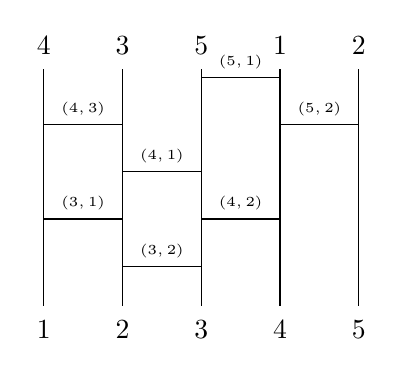
\begin{tikzpicture}
		 	\draw(0, 0) to (0, 3);
		 		\draw(0, 2.3) to (1, 2.3);
		 		\draw(0, 1.1) to (1, 1.1);

		 	\draw(1, 0) to (1, 3);
				 \draw(1, 1.7) to (2, 1.7);
				 \draw(1, .5) to (2, .5);
		 	\draw(2, 0) to (2, 3);
				 \draw(2, 2.9) to (3, 2.9);
				 \draw(2, 1.1) to (3, 1.1);
			 \draw(3, 0) to (3, 3);
			 	\draw(3, 2.3) to (4, 2.3);
			 \draw(4,0) to (4, 3);

			 \node at(0, 3.3){$4$};
			 \node at(1, 3.3){$3$};
			 \node at(2, 3.3){$5$};
			 \node at(3, 3.3){$1$};
			 \node at(4, 3.3){$2$};
			 \node at(0, -.3){$1$};
			 \node at(1, -.3){$2$};
			 \node at(2, -.3){$3$};
			 \node at(3, -.3){$4$};
			 \node at(4, -.3){$5$};

			 \node at(.5, 2.5){\tiny{$(4,3)$}};
			 \node at(.5, 1.3){\tiny{$(3,1)$}};
			 \node at(1.5, 1.9){\tiny{$(4,1)$}};
			 \node at(1.5, .7){\tiny{$(3,2)$}};
			 \node at(2.5, 3.1){\tiny{$(5,1)$}};
			 \node at(2.5, 1.3){\tiny{$(4,2)$}};
			 \node at(3.5, 2.5){\tiny{$(5,2)$}};


		\end{tikzpicture}
				

	\end{minipage}
	\begin{minipage}{.4\textwidth}
		\begin{flushright}
		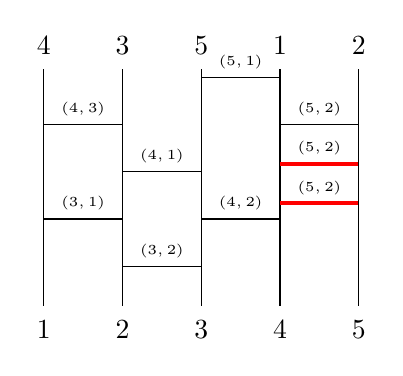
\begin{tikzpicture}
		 	\draw(0, 0) to (0, 3);
		 		\draw(0, 2.3) to (1, 2.3);
		 		\draw(0, 1.1) to (1, 1.1);

		 	\draw(1, 0) to (1, 3);
				 \draw(1, 1.7) to (2, 1.7);
				 \draw(1, .5) to (2, .5);
		 	\draw(2, 0) to (2, 3);
				 \draw(2, 2.9) to (3, 2.9);
				 \draw(2, 1.1) to (3, 1.1);
			 \draw(3, 0) to (3, 3);
				 \draw(3, 2.3) to (4, 2.3);
				 \draw [line width=0.5mm, red ](3, 1.8) to (4, 1.8);
				 \draw[line width=0.5mm, red ](3, 1.3) to (4, 1.3);
			 \draw(4,0) to (4, 3);

			 \node at(0, 3.3){$4$};
			 \node at(1, 3.3){$3$};
			 \node at(2, 3.3){$5$};
			 \node at(3, 3.3){$1$};
			 \node at(4, 3.3){$2$};
			 \node at(0, -.3){$1$};
			 \node at(1, -.3){$2$};
			 \node at(2, -.3){$3$};
			 \node at(3, -.3){$4$};
			 \node at(4, -.3){$5$};


			 \node at(.5, 2.5){\tiny{$(4,3)$}};
			 \node at(.5, 1.3){\tiny{$(3,1)$}};
			 \node at(1.5, 1.9){\tiny{$(4,1)$}};
			 \node at(1.5, .7){\tiny{$(3,2)$}};
			 \node at(2.5, 3.1){\tiny{$(5,1)$}};
			 \node at(2.5, 1.3){\tiny{$(4,2)$}};
			 \node at(3.5, 2.5){\tiny{$(5,2)$}};
			 \node at(3.5, 2.0){\tiny{$(5,2)$}};
			 \node at(3.5, 1.5){\tiny{$(5,2)$}};



		\end{tikzpicture}
	\end{flushright}
	\end{minipage}
	\caption{Two ladders for the permutation $(4,3,5,1,2)$. The left ladder is an optimal ladder and the right ladder is not. 
	The bold  bars in the right ladder are redundant, thus the right ladder is non optimal.}
	\label{fig:ab}
\end{figure}
Let $OptL\{\pi\}$ be defined as the set of optimal ladder lotteries that form an equivalence class 
insofar as all ladders in $OptL\{\pi\}$ sort $\pi$ in ascending order with the least number of bars.
Let $k$ be the number of bars in a ladder such that $k$ equals the number of inversions 
in $\pi$.  Assume there is one row in the ladder for each of the $k$ bars; thus there are $k$ rows in the ladder. Let $\pi$ be of order $n$.
There $n-1$ columns, gaps between lines, in the ladder to place bars. Hence, the dimensions of the ladder associated with $\pi$
are $(n-1)$ by $(k)$. The total number of ladders with $(n-1)$ columns and $k$ rows is ${(n-1)(k) \choose k}$ which is finite. 
For each optimal ladder lottery with $(n-1)$ columns and $k$ bars, their aggregation forms a subset of 
all ${(n-1)(k) \choose k}$ ladder lotteries known as $OptL\{\pi\}$. Therefore, $OptL\{\pi\}$ is finite. 
Generating $OptL\{\pi\}$ was essential for producing the sample data for this thesis. The first discussion of 
$OptL\{\pi\}$ is in the paper Efficient Enumeration of Ladder Lotteries and its Application~\cite{A1}.
In this paper, the authors provide an algorithm known as {\sc FindAllChildren}
which generates $OptL\{\pi\}$; the details of the algorithm are discussed in Chapter 2.
To see $OptL\{(4,3,5,1,2)\}$ please refer to Figure \ref{Fig:OptL3421}.
Given that there are $n!$ permutations of order $n$, each of them 
have their own $OptL\{\pi\}$. In Table~\ref{Table:125} found in the appendix, 
the number of ladders in each of the 120 $OptL\{\pi\}$ of order $5$ is presented.
\begin{figure}[h]
	\centering
	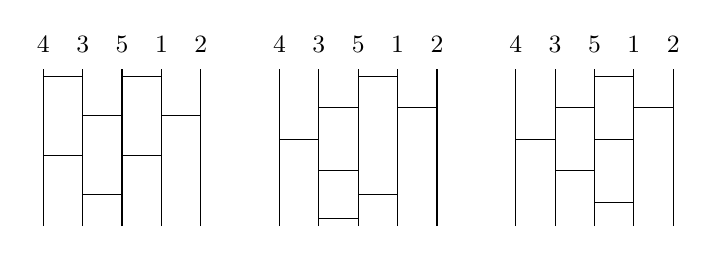
\begin{tikzpicture}
		\draw(0,0) to (0,2);
			\draw(0, 1.9) to (.5, 1.9);
			\draw(0, .9) to (.5, .9);
		\draw(.5,0) to (0.5,2);
			\draw(.5, 1.4) to (1, 1.4);
			\draw(.5, .4) to (1, .4);
		\draw(1,0) to (1,2);
			\draw(1, 1.9) to (1.5, 1.9);
			\draw(1, .9) to (1.5, .9);
		\draw(1.5,0) to (1.5,2);
			\draw(1.5, 1.4) to (2, 1.4);
		\draw(2,0) to (2,2);

		\draw(3, 0) to (3, 2);
			\draw(4, 1.9) to (4.5, 1.9);
			\draw(3.5, 1.5) to (4, 1.5);
			\draw(4.5, 1.5) to (5, 1.5);
			\draw(3.5, 1.1) to (3, 1.1);
			\draw(3.5, 0.7) to (4, 0.7);
			\draw(4, .4) to (4.5, .4);
			\draw(3.5, .1) to (4, .1);
		\draw(3.5, 0) to (3.5, 2);
		\draw(4, 0) to (4, 2);
		\draw(4.5, 0) to (4.5, 2);
		\draw(5, 0) to (5, 2);

		\draw(6, 0) to (6, 2);
			\draw(7.5, 1.9) to (7, 1.9);
			\draw(6.5, 1.5) to (7, 1.5);
			\draw(7.5, 1.5) to (8, 1.5);
			\draw(6, 1.1) to (6.5, 1.1);
			\draw(7, 1.1) to (7.5, 1.1);
			\draw(6.5, 0.7) to (7, 0.7);
			\draw(7, 0.3) to (7.5, 0.3);
		\draw(6.5, 0) to (6.5, 2);
		\draw(7, 0) to (7, 2);
		\draw(7.5, 0) to (7.5, 2);
		\draw(8, 0) to (8, 2);

		\node at(0, 2.3){\small{$4$}};
		\node at(.5, 2.3){\small{$3$}};
		\node at(1, 2.3){\small{$5$}};
		\node at(1.5, 2.3){\small{$1$}};
		\node at(2, 2.3){\small{$2$}};

		\node at(3, 2.3){\small{$4$}};
		\node at(3.5, 2.3){\small{$3$}};
		\node at(4, 2.3){\small{$5$}};
		\node at(4.5, 2.3){\small{$1$}};
		\node at(5, 2.3){\small{$2$}};

		\node at(6, 2.3){\small{$4$}};
		\node at(6.5, 2.3){\small{$3$}};
		\node at(7, 2.3){\small{$5$}};
		\node at(7.5, 2.3){\small{$1$}};
		\node at(8, 2.3){\small{$2$}};
	\end{tikzpicture}
	\caption{All the optimal ladders in $OptL\{(4,3,5,1,2)\}$}
	\label{Fig:OptL3421}
\end{figure}

Research on ladder lotteries falls under research in \emph{combinatorial generation}. Combinatorial 
generation is a subfield of theoretical computer science which pertains to listing 
all combinatorial objects such as permutations, combinations, sets, subsets and graphs. Gray codes are a 
special type of combinatorial generation in which a minimal amount of constant change 
is required to get from one object to the next. For example, a single swap operation,
a single rotation, or a single bit negation is used to get from one object to the next. Some examples of Gray Codes 
are the Binary Reflected Gray Code, De Bruijn sequence, Steinhaus-Johnson-Trotter's algorithm and 
Snake-in-the-box codes.\par 
Much research has been done on combinatorial generation, especially 
in regards to generating permutations. Throughout the course of this thesis,
a number of permutation generating algorithms were researched~\cite{A18}\cite{A19}\cite{A21}\cite{A24}\cite{A25}\cite{A26}\cite{A31}\cite{A34}\cite{A35}s.
After considering these algorithms, two were considered the most beneficial for this thesis. 
These algorithms are the Effler-Ruskey algorithm and the Steinhaus-Johnson–Trotter algorithm found in~\cite{A26}\cite{A25}.
The reason these two algorithms were considered the most beneficial is because of 
their efficiency. The Effler-Ruskey algorithm is a backtracking algorithm and the Steinhaus-Johnson-Trotter 
is a Gray Code. In this thesis, modifications to these algorithms are done such that the 
modified algorithms are applied to ladder lotteries. Thus, this thesis provides further knowledge 
in the field of combinatorial generation by providing novel algorithms for generating ladder lotteries.\par 
The motivation for this thesis is to provide more knowledge to the field of combinatorics and combinatorial 
generation. In this thesis, the aforementioned permutation listing algorithms are modified in order to 
list $n!$ ladder lotteries, each of which corresponds to one of the $n!$ permutations of order $n$.
The second problem which this thesis focuses on is the so called Minimum Height Problem which is an optimization 
problem. Optimization problems are widely studied in computer science. Optimization problems are found in 
the fields of artificial intelligence, theory of computation and machine learning. Let the 
\emph{height of the ladder} be defined as the number of non-empty rows in the ladder data structure. We know 
that with $OptL\{\pi\}$, the ladders in the set form an equivalence class. Thus, the goal is to create 
the ladder from $OptL\{\pi\}$ with the minimum height; i.e. the minimum number of rows. The reason 
for doing so is that the implementation of a ladder with the minimum height allows for equivalent behavior 
as any other ladder in the set, while being the most space efficient. In Figure \ref{Fig:OptL3421}, the leftmost 
ladder has the minimal height with a height of $4$.



\section{Thesis Statement}
  	This thesis considers two problems related 
    to ladder lotteries. The first problem is the so called Canonical Ladder Listing Problem. 
	This problem asks, given all $n!$ permutations of order $n$, is there an efficient algorithm for listing 
	one optimal ladder per permutation? In other words, 
	is there an easy way to transition from one ladder to the next until all $n!$ ladders 
	have been listed? Efficiency is defined as relocating the minimal number of bars in $ladder_{i}$ 
	to get to $ladder_{i+1}$ or add/removing the minimal number of bars in $ladder_{i}$
	to get to $ladder_{i+1}$. This thesis provides two such algorithms for solving the Canonical
	Ladder Listing Problem. The first is a modification of the Steinhaus-Johnson-Trotter Gray Code. The second 
	is a modification of the Effler-Ruskey algorithm.\par  
	The second problem is the so called Minimum Height 
    Problem which asks, given all the ladders in $OptL\{\pi\}$, which ladder(s) are 
    the shortest? That is to say, which ladders have the least number of rows? Furthermore, given some arbitrary $\pi$, 
	is there an efficient algorithm to create a ladder for $\pi$ with minimal height? Efficiency is defined as 
	$O(n^{2})$. This thesis provides an upper and lower bound for the minimal height of ladders along with an efficient heuristic algorithm 
	for creating a ladder with minimal height. The heuristic algorithm uses the properties of bar compression and zig-zagginess 
	in order to create a ladder with minimal height.
	
\section{Overview of Thesis}
This thesis is broken down into several sections. In Chapter 2, a literature
review of ladder lotteries will be provided along with background information pertinent to this thesis. 
The literature review focuses on solved problems pertaining 
to ladder lotteries along with the commonalities between ladder lotteries and 
other mathematical objects. In Chapter 3, The Canonical Ladder Listing Problem is provided. 
Chapter 3 is broken down into four subsections. The first subsection is the introduction to the problem, 
the second is a methodology subsection, the third is a results 
subsection and the fourth is a conclusion/analysis subsection. The introduction subsection introduces the problem to the reader, providing the necessary 
definitions and concepts. The methodology subsection provides the modified SJT algorithm and the modified Effler-Ruskey algorithm pertaining 
to listing ladder lotteries. 
Following the methodology subsection, the results generated by the algorithms will be presented.
In the results subsection there will be proofs and formulas for certain propositions made in regards to the Ladder Lottery Listing Problem. 
Following the results subsection, an analysis of the results will be presented along with a summary of future work. 
In Chapter 4, The Minimum Height Problem is provided. Chapter 4 is broken down into four subsections.
The first subsection is the introduction to the problem, 
the second is a methodology subsection, the third is a results 
subsection and the fourth is a conclusion/analysis subsection.
The introduction subsection introduces the problem to the reader, providing the necessary concepts and definitions. The 
introduction subsection also connects ladders of minimum height to a number of other mathematical objects such as 
involutions and binary strings; details can be found in Chapter 4 subsection introduction. The second subsection 
is the procedure subsection which provides a number of algorithms for solving the minimum height problem. One is an exact 
algorithm for solving the minimum height problem given a descending permutation of order $n$. The second is a heuristic 
algorithm for solving the minimum height problem for an arbitrary permutation of order $n$. There are also a number 
of lemmas and proofs in the procedure subsection pertaining to the Minimum Height Problem. In the results subsection, 
the results of the heuristic algorithm for solving the Minimum 
Height Problem are provided. In the analysis subsection, the results of the heuristic algorithm are compared with the results of the brute 
force algorithm. 

\section{Summary of Past Known Results}
To the best of my knowledge, the first paper written on ladder lotteries is titled Efficient Enumeration of 
Ladder Lotteries and its Application written by Yamanaka, Nakano, Matsui Uehara and Nakada. The paper 
was written in 2010~\cite{A1}. Since this paper, 
a number of problems related to ladder lotteries have been solved. In Table~\ref{Table:KnownProblems} 
the reader will find a table of solved problems related to ladder lotteries. In Chapter 2 a more comprehensive analysis of these 
solved problems will be provided.
\begin{table}[h]
	\centering
	\begin{tabular}{|p{4cm}||p{4cm}||p{4cm}|}
		\hline 
		\multicolumn{3}{|c|}{Table of Known Results Related to Ladder Lotteries}\\
		\hline 
		\hline 
		Name of Problem & Description & Source \\ 
		\hline 
		\small{Enumeration Problem} & \small{Generates $OptL\{\pi\}$} &~\cite{A1} 2010\\ 
		\hline
		\small{Ladder Lottery \newline Realization Problem} & \small{Determines time complexity for creating a ladder lottery given a multi-set of bars} &~\cite{A3} 2018\\ 
		\hline
		\small{The Reconfiguration \newline Problem} & \small{Determine the length of the path between two ladders in $OptL\{\pi\}$} &~\cite{A2} 2017\\ 
		\hline 
		\small{Enumeration Problem \newline given $n$, $k$} & \small{Generates all ladders with $n$ lines and $k$ bars; includes non-optimal ladders} &~\cite{A4} 2014\\ 
		\hline
		\small{The Coding Problem} & \small{Provides a binary string encoding for a ladder lottery} &~\cite{A5} 2012\\ 
		\hline 
		\small{Counting and \newline Random Generation \newline Problem} & \small{Provides a solution for counting ladder lotteries of a given type as well as randomly generating a ladder lottery} &~\cite{A6} 2017\\ 
		\hline
		
																



	\end{tabular}
	\caption{Table of known solutions for problems related to ladder lotteries}
	\label{Table:KnownProblems}
\end{table}